%Centralizar verticalmente.
\newenvironment{midpage}{\vspace*{\fill}}{\vspace*{\fill}}
%Centralizar horizontalmente.
\newenvironment{midline}{\hspace*{\fill}}{\hspace*{\fill}}
\documentclass[12pts]{article}
\usepackage[utf8]{inputenc}
%Pacote para colocar cor no código.
\usepackage{color}
\definecolor{light-gray}{gray}{0.95}
%Pacote para inserir código.
\usepackage{listings}
\lstset{
    numbers=left,
    tabsize=2,
    backgroundcolor=\color{light-gray},
}
\title{
	Prática de Eletrônica Digital 1 - (119466)
	\singlespacing
		Turma E (Unb - Gama)
	\singlespacing
	\begin{midpage}
	\begin {large}
		Pré-Relatório Experimento 7
		\singlespace
		Circuitos Contadores Síncronos e Assíncronos
	\end {large}
	\end{midpage}
}
\date{Novembro 7, 2016}
\usepackage{indentfirst}
\usepackage{setspace}
\usepackage{verbatim}
\usepackage[pdftex]{hyperref}
\usepackage{graphicx}
\begin{document}
\maketitle	
%\vspace{100 mm}
\begin{center}

\begin{tabular}{|c|l|r|}
\hline
Nome & Matrícula & Assinatura\\
\hline
Arthur Temporim & 14/0016759 & \\
\hline	
Eduardo Nunes & 14/0056149 & \\
\hline	
\end{tabular}

\end{center}

\pagebreak

\section{Pesquisa bibliográfica}

	Na seção a seguir contém as atividades pedidas para a elaboração do pré-relatório.
\singlespacing
\textit{\textbf{A)} Quais são os principais problemas existentes nos contadores assíncronos? Descreva cada um deles de forma resumida.}
\singlespacing

Os problemas encontrados com os contadores assíncronos são provocados pelo acúmulo dos atrasos de propagação dos Flip Flops.

\begin{figure}[!htb]
  \centering
  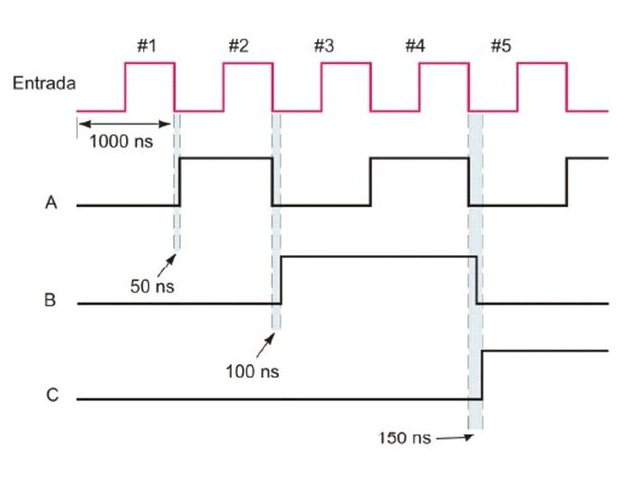
\includegraphics[scale=0.4]{imagens/oi.png}
  \caption{Exemplo de atraso de propagação}
  \label{figRotulo}
\end{figure}


Na imagem acima, está uma possível representação do impacto destes atraso. Pois, o tempo de atraso é de 50ns como os pulsos de entrada ocorrem a cada 100 ns na transição de 1 para 0. Na segunda transição este atraso tem seu valor dobrado, uma vez que, se soma o valor do primeiro atraso com o do segundo atraso, ou seja o atraso é acumulado. E por consequência, na terceira transição não foi contado o pulso que foi acionado, uma vez que, o tempo de atraso, sendo este agora de 150 ns, acabou por não captar o pulso.  

\pagebreak
\textit{\textbf{B)} Cite as vantagens dos contadores síncronos em relação aos contadores assíncronos.}
\singlespacing

Dado a problemática do exercício anterior dos atrasos de propagação, os contadores síncronos podem solucionar este problema, nos quais os FFs são disparados simulataneamente (em paralelo) pelos pulsos de clock de entrada. Porém, mesmo com a utilização dos contadores síncronos ainda haverá atrasos de propagação no entanto estes sem bem inferiores aos atrasos ocorridos nos contadores assincronos. 

\singlespacing
\textit{\textbf{C)} Realize um resumo do procedimento para a realização de projeto de circuitos contadores sincronos e assincronos. Procure deixar bem claro as diferenças no procedimento nos dois tipos de circuitos.}
\singlespacing

Na criação de um projeto de um contador assíncrono considera se que as entradas J e K dos FFs estejam com o nivel alto permantemente, ou seja 1, e que a saída de um FF é ligada a entrada de clock do FF seguinte. Já no projeto de um contador síncrono somente as entradas J e K do primeiro FF estão no nível alto e as dos outros FF estão conectadas com uma combinação de saídas dos outros FFs. E as entradas CLK dos FF estão ligadas juntas de forma que na hora que o clock for acionando todas acionam simultaneamente. Desta forma um contador sincrono precisa de mais circuito que um contador assincrono.

\singlespacing
\textit{\textbf{D)} Descreva aplicações práticas que utilizam os circuitos contadores.}

\singlespacing
Uma das aplicações comuns é o sistema de contagem de tempo empregado nos relógios digitais. Um relógio digital mostra horas, minutos e segundos. Primeiramente, uma tensão de 60 Hz (60 pulsos por segundo) é convertida em forma de onda e dividida para forma de pulsos de 1 Hz (1 pulso por segundo). Para segundos e minutos é empregado um contador de 0 a 59 e para horas, de 0 a 12. Para cada pulso de 1 Hz o display apresenta sua contagem. O contador de segundos gera um clock para o contador de minutos, que gera um clock para o contador de horas. O contador de segundos e minutos contam de 0 a 59 e, em seguida, se reciclam para 0. São utilizados contadores de décadas síncronos.

\singlespacing
\textbf{Referências:}
\singlespacing
Exemplo de aplicação retirado do site: wikipedia.org/wiki/Contadores\_digitais
Imagem utilizada na questão 01: slideplayer.com.br/slide/364035/
\singlespacing

\pagebreak
\section{Projetos e simulações}

\subsection{Projeto 1}

Este projeto consiste em um contador sincrono com um \textit{reset} assincrono. Ele conta de 0 a 9 de forma crescente e decrescente de acordo com o valor da entrada "direcao".

\subsubsection{Código VHDL}
\lstinputlisting[language=vhdl]{projetos/projeto1/projeto1.vhd}                                                                                                                                     

\subsubsection{Diagrama de Ondas}
	\begin{figure}[!htb]
	  \centering
	  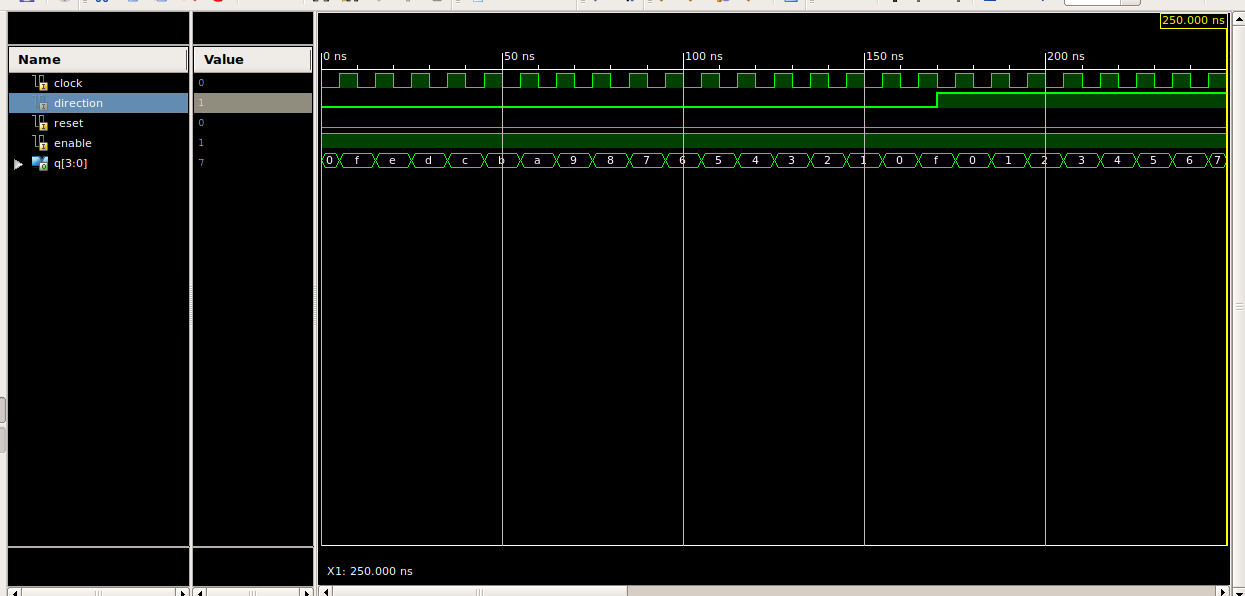
\includegraphics[scale=0.38]{imagens/onda_projeto_1.png}
	  \caption{Diagrama de ondas 1 - ISE Design Suit 14.7}
	  \label{figRotulo}
	\end{figure}

\pagebreak
\subsection{Projeto 2}

Este projeto consiste em um contador sincrono com um \textit{reset} assincrono. Ele conta na sequência: \textbf{0,2,5,6}. É possível também inserir outros valores no intervalo de 0 a 6, caso o valor não esteja na contagem, o circuito automáticamente volta para o estado "0". 

Diferente do projeto anterior, este circuito foi programado na forma de máquina de estados.

\subsubsection{Código VHDL}
\lstinputlisting[language=vhdl]{projetos/projeto1/projeto_2.vhd}                                                                                                                                     
\subsubsection{Diagrama de Ondas}
	\begin{figure}[!htb]
	  \centering
	  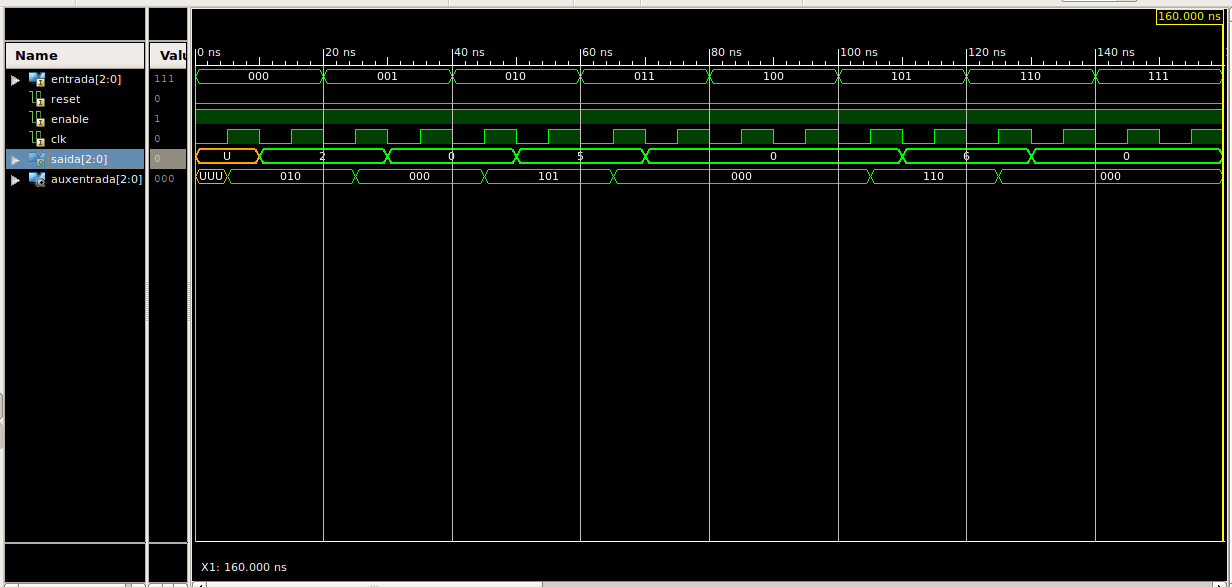
\includegraphics[scale=0.38]{imagens/onda_projeto_2.png}
	  \caption{Diagrama de ondas 2 - ISE Design Suit 14.7}
	  \label{figRotulo}
	\end{figure}
\end{document}
